% -*- coding: utf-8 -*-
%

% reset all acronym expansions
\acresetall

%%%%%%%%%%%%%%%%%%%%%%%%%%%%%%%%%%%%%%%%%%%%%%
\chapter{Evaluation}
\label{ch:Evaluation}
%%%%%%%%%%%%%%%%%%%%%%%%%%%%%%%%%%%%%%%%%%%%%%

In this Chapter we describe the experiments that were conducted regarding the implementation of \ac{ml} algorithms using privacy-preserving techniques made to prove the concept of the platform. In Section \ref{sec:EvaluationMetrics}, we present the metrics used in the experiments. Section \ref{sec:ExperimentalSetup} describes the setup that was used to run the experiments, as well as the toolkits used and the parameters chosen for those toolkits. In Section \ref{sec:ExperimentalResultsBaseline}, we present the best baseline results obtained for the datasets in question and in Section \ref{sec:ExperimentalResultsComparisonBaseline} we compare those results with the ones obtained using the toolkits. In Section \ref{sec:ExperimentalResultsExecutionTime}, we present the execution times for the combinations of \ac{ml} algorithms and privacy-preserving techniques that were implemented. In Section \ref{sec:CommunicationCosts} we present the communication costs for those combinations. Finally, in Section \ref{sec:ExperimentalResultsConclusion} we make some final observations about the obtained results.


  %%%%%%%%%%%%%%%%%%%%%%%%%%%%%%%%%%%%%%%%%%%%%%%%%%%%%%%%%%%%%%%%%%%%%%%%%%%%%
  %
%%%%%                        THE BEGINNING
 %%%
  %

\section{Evaluation Metrics}
\label{sec:EvaluationMetrics}

To evaluate our implementation, a set of metrics was considered, namely: \emph{accuracy}, \emph{precision}, \emph{recall}, and \emph{F-measure}. For the definition of the metrics, we need to define the events that can occur when making predictions, shown in Table \ref{table:notation} below. 
\begin{table}[htp]
\centering
\caption{Binary confusion matrix.}
\label{table:notation}
\vspace*{0.2cm}
\begin{tabular}{cc|c|c|} 
\cline{3-3}\cline{4-4}
                                                         &    & \multicolumn{2}{c|}{\textbf{Real label}}                             \\ 
\cline{3-3}\cline{4-4}
                                                         &    & +1                              & -1                        \\ 
\hline
\multicolumn{1}{|c|}{\multirow{2}{*}{\textbf{Predicted label}~~}} & +1 & \ac{tp}        & \ac{fp}  \\ 
\cline{2-4}
\multicolumn{1}{|l|}{}                                   & -1 & \ac{fn}        & \ac{tn}  \\
\hline
\end{tabular}
\end{table}




\textit{Accuracy} is defined as how much of the measurements of a value differ to the real value. In our implementation, it represents how many times the predictions calculated by the \ac{ml} generated models match the class of the testing samples. In mathematical terms, it is represented by:
\begin{equation}
\label{eq:accuracy}
accuracy=\frac{TP + TN} {TP + TN + FP + FN} 
\end{equation}


\textit{Precision} is defined by the fraction of relevant instances among the retrieved instances. \textit{Recall} is defined by the fraction of relevant instances that have been retrieved over the total of the relevant instances.
\begin{equation}
\label{eq:precision}
precision=\frac{TP}{TP + FP}
\end{equation}
\begin{equation}
\label{eq:recall}
recall=\frac{TP}{TP + FN}
\end{equation}

\textit{F-measure} is a measure of the accuracy of a test. It considers both the precision and the recall of the test to compute the score:
\begin{equation}
\label{eq:f-measure}
F_1=2\centerdot \frac{precision\centerdot recall}{precision + recall}
\end{equation}



Besides these metrics, we also used additional ones in order to understand how much the computational overhead due to the use of cryptography influences the system.
We compared the \emph{results} obtained by the privacy-preserving versions of \ac{ml} algorithms with the ones obtained using the baseline. We also take into account the \emph{execution times} of the system, which shows the overhead caused by the additional computational cost added by cryptography.
Finally, we also show the increase in communication costs that happen when cryptography is involved, as all values must be represented by ciphertext, instead of plaintext integer or float values.


%%%%%%%%%%%%%%%%%%%%%%%%%%%%%%%%%%%%%%%%%%%%%%
\section{Experimental Setup}
\label{sec:ExperimentalSetup}
%%%%%%%%%%%%%%%%%%%%%%%%%%%%%%%%%%%%%%%%%%%%%%

All the experiments were performed using a machine with an Intel Core i5-4300M CPU @2.60Gz with 3MB L3 cache memory and 12 GB RAM memory.

For obtaining the experimental results, we started by applying the preprocessing techniques mentioned in Section \ref{sec:DataPreProcessingImplementation} to the datasets described in Table \ref{table:datasets}. As described before, all datasets that were composed of a single file were split into three sets: training, validation and testing sets, with the proportion $70/15/15$. Each \ac{ml} model was trained using the training set, the best model configuration was chosen using the validation set, and the model performance was evaluated using the testing set.

Taking into account that the baseline implementation was done using \textit{scikit-learn}, we could not explicitly observe the operations done in the toolkit since they were made in a black box. This could lead to an inability to distinguish prediction errors caused by the privacy-preserving systems and caused by the implementation of the prediction equations. To solve this problem, we implemented the prediction processes of the \ac{ml} algorithms without using the toolkit, i.e. directly from the algorithm equations.
We successfully recreated the prediction processes by retrieving from the toolkit the specifications for each \ac{ml} model.

\begin{itemize}
  
    \item For the \ac{dt}, we needed to retrieve all of the model, i.e. the binary tree, so that we could traverse it according to each testing sample, comparing the feature with the threshold of each node, and choosing which branch of the tree to follow, until a label is reached. 

    \item In the case of \ac{svm}, we retrieved from the toolkit all the coefficients needed to compute Equation \ref{eq:SVM3}, namely the support vectors $x_{SV}^{(i)}$, the $\alpha_i$ coefficients for each support vector, the kernel function $k({\vec {x_{i}}},{\vec {x_{j}}})$ that was used (linear or polynomial), the exponent for the polynomial kernel if needed, and the scalar value $b$.

    %\item In the case of \ac{k-nn}, since training does not exist, there was no need to use the toolkit, so no information was retrieved from it, and it was not required to do an expanded version of the algorithm.

    \item For \ac{k-m}, we just required from the toolkit the centroids for each cluster, as well as the prediction labels associated with each one. The classification of each testing sample was done by discovering which centroid was closest to it.

    \item In \ac{lr}, we extracted the $\beta=(\beta_0,\beta_1,...,\beta_n)$ that appear in Equation \ref{eq:LR3}. $\beta_0$ is the intercept from the linear regression, and $\beta_i$ are each regression coefficient that are multiplied by each feature of the sample.

\end{itemize}


\subsection{Baseline Parameters}

The following parameters are the ones used in the \textit{scikit-learn} toolkit.

For the experiments with \ac{dt}, we tested the values for \textit{max\textunderscore depth} of 5\%, 10\%, 20\%, 50\%, 100\%, 200\%, and 500\% of the total number of features, and the values for \textit{min\textunderscore samples\textunderscore leaf} of 0.001\%, 0.002\%, 0.005\%, 0.01\%, 0.02\%, 0.05\%, 0.1\%, 0.2\%, 0.5\%, 1\%, 2\% and 5\% of the total number of training samples.

For the experiments with \ac{svm}, we used \textit{kernel} values of \textit{linear}, \textit{poly} and \textit{rbf}. For all kernels, we used $C$ values of $2^{-10}$, $2^{-6}$, $2^{-2}$, $2^{2}$, $2^{6}$ and $2^{10}$. For the polynomial kernel, we used \textit{degree} values of 2, 3 and 4. For the \ac{rbf} kernel, we used $\gamma$ values of $2^{-9}$, $2^{-5}$, $2^{-1}$, $2^{1}$ and $2^{3}$.

For the experiments with \ac{k-m}, we tested with a variable number of clusters, i.e. with \textit{num\textunderscore clusters} values of 2, 3, 4, 5, 6, 7, 8, 9, 10, 20, 30, 40, 50, 60, 70, 80, 90 and 100.

For the experiments with \ac{lr}, we used the \textit{liblinear} solver with $C$ values of $2^{-10}$, $2^{-6}$, $2^{-2}$, $2^{2}$, $2^{6}$ and $2^{10}$.

 These variations on parameters allowed to train models with all possible configurations without the need to specifically adapt the parameters to the different datasets.





\subsection{\acl{gc} toolkits and parameters}

For the experiments with \ac{gc}, we used the toolkit developed by VIPP group from the University of Siena\footnote{\url{http://clem.dii.unisi.it/~vipp/index.php/home}}. This toolkit was not our first choice since it has known issues in computation times, but the other toolkits that we tested contained limitations that we could not overcome, as stated below:
\begin{itemize}
    
    \item\textbf{ABY\cite{demmler2015aby}:} We found it impossible to define gate-to-gate wires, and that removed the ability for fine control on how to use and combine wires.

    \item\textbf{JustGarble\cite{bellare2013efficient}:} This toolkit could not be fully compiled due to conflicts with current versions of the GNU gcc compiler.

    \item\textbf{Ciphermed\cite{bost2015machine}:} This toolkit is efficient for small \ac{dt}, but is exponentially slower for larger trees (above 10 nodes).

    \item\textbf{TinyGarble\cite{songhori2015tinygarble}:} The current version of this toolkit does not support the open source synthesis tool (Yosis\footnote{\url{http://www.clifford.at/yosys/}}) recommended by the authors, and only supports a paid one.

    \item\textbf{CompGC\cite{groce2016compgc}:} The implementation of all the examples of \ac{ml} algorithms in this toolkit are hardcoded, making it extremely difficult to adapt to our needs.

\end{itemize}

In the experiments using \ac{gc}, we tested values of 8, 12, 16, 20 and 24 bits for the numeric precision of the data and model parameters. This will be reflected in the circuit size and the accuracy of the results. Larger values were not considered because 24 bits are already sufficient for an exact representation of the input values and model parameters.

\subsection{\acl{he} toolkits and parameters}

For the experiments using \ac{phe}, we implemented our own version of the Paillier cryptosystem \cite{paillier1999public}. We decided to do this way instead of using an existing toolkit because it was simple to implement and because it provided a good learning experience on the inner workings of a cryptographic system.

For the experiments using \ac{fhe}, we used the HElib toolkit \cite{halevi2014helib}. Two methods were considered in the implementation, method M1: multiply and sum arrays without packing, and method M2: use coefficient packing, invert and multiply polynomials, that was inspired in a HElib tutorial\footnote{\url{https://mshcruz.wordpress.com/2016/09/27/scalar-product-using-helib/}}. It is also important to note that, due to intrinsic limitations in HElib, we had to pre-compute $\alpha_i\centerdot x_{SV}^{(i)}$ when evaluating the \ac{svm}. However, this does not negatively affect the experiments, since these model parameters are both owned by the same party.

For the experiments using \ac{phe}, we used the values of 128, 256, 512, 1024 and 2048 bits (NBits) for the length of the cryptographic keys.

For the experiments using \ac{fhe}, no parameter search was made, since adequate default values were pre-determined for most parameters, and we chose a large enough number for the modulus ($(2^{15})^4=2^{60}$). Changing these parameters should not affect the obtained predicted labels in any way, although they may have minimal effects on the actual output of the evaluation functions of \ac{lr} and \ac{svm} algorithms. The values considered are too large to affect the results and correspond to a cryptographic security factor.


%%%%%%%%%%%%%%%%%%%%%%%%%%%%%%%%%%%%%%%%%%%%%%
\section{Baseline Results}
\label{sec:ExperimentalResultsBaseline}
%%%%%%%%%%%%%%%%%%%%%%%%%%%%%%%%%%%%%%%%%%%%%%


We now show the experimental results obtained by applying different \ac{ml} algorithms to the datasets mentioned above.
In terms of execution time results for the baseline, we were able to observe that they are in the order of milliseconds per data sample.

In each Section below, for each dataset, we present the different \ac{ml} algorithms and parameters. The results shown in the following tables are the ones obtained in the testing sets using the parameters that provided the best accuracy or F-Measure results with the validation set. We also present results found in the literature, for comparison.

\subsection{\emph{Pima Indians Diabetes} Dataset}

We present the best baseline results obtained in the testing set for the \emph{Pima Indians Diabetes} Dataset in Table \ref{table:baselinePID}. We can see that our results are comparable to the ones found in the literature.

\begin{table}[htp]
\centering
\caption{Baseline results, in percentage. \emph{Pima Indians Diabetes} Dataset. ``A'' represents Accuracy, ``F'' represents F-Measure.}
\label{table:baselinePID}
\vspace*{0.2cm}
\begin{tabular}{|l|c|c|c|c|c|c|}
\hline
\multirow{1}{*}{\textbf{ML}} & \multirow{2}{*}{\textbf{DT}} & \multirow{2}{*}{\textbf{k-Means}} & \multirow{2}{*}{\textbf{LR}} & \multicolumn{3}{c|}{\textbf{SVM}} \\ \cline{5-7} 
\textbf{algorithm} &  &  & & Linear & Poly & RBF  \\ \hline
Baseline & \begin{tabular}[c]{@{}l@{}}A: 73.04\\   F: 63.53\end{tabular} & \begin{tabular}[c]{@{}l@{}}A: 72.17\\ F: 52.94\end{tabular} & \begin{tabular}[c]{@{}l@{}}A: 75.65\\   F: 58.82\end{tabular} & \begin{tabular}[c]{@{}l@{}}A: 75.65\\   F: 61.11\end{tabular} & \begin{tabular}[c]{@{}l@{}}A: 76.52\\   F: 59.70\end{tabular} & \begin{tabular}[c]{@{}l@{}}A: 77.39\\   F: 62.86\end{tabular}  \\ \hline

Literature  & \begin{tabular}[c]{@{}l@{}}A: 75.39\cite{anwar2014global}\\   F: -\end{tabular} & \begin{tabular}[c]{@{}l@{}}A: 73.7\cite{eggermont2004genetic}\\   F: -\end{tabular}  & \begin{tabular}[c]{@{}l@{}}A: 77.95\cite{anwar2014global}\\   F: -\end{tabular} & \begin{tabular}[c]{@{}l@{}}A: -\\   F: -\end{tabular} & \begin{tabular}[c]{@{}l@{}}A: -\\   F: -\end{tabular} & \begin{tabular}[c]{@{}l@{}}A: 80.2\cite{abdillah2016diagnosis}\\   F: -\end{tabular} \\ \hline
\end{tabular}
\end{table}

\subsection{\emph{Breast Cancer Wisconsin Diagnostic} Dataset}

We present the best baseline results obtained in the testing set for the \emph{Breast Cancer Wisconsin Diagnostic} Dataset in Table \ref{table:baselineBCW}. As we see, our baseline results are, again, close to the ones found in the literature.

\begin{table}[htp]
\centering
\caption{Baseline results, in percentage. \emph{Breast Cancer Wisconsin Diagnostic} Dataset. ``A'' represents Accuracy, ``F'' represents F-Measure.}
\label{table:baselineBCW}
\vspace*{0.2cm}
\begin{tabular}{|l|c|c|c|c|c|c|}
\hline
\multirow{1}{*}{\textbf{ML}} & \multirow{2}{*}{\textbf{DT}} & \multirow{2}{*}{\textbf{k-Means}} & \multirow{2}{*}{\textbf{LR}} & \multicolumn{3}{c|}{\textbf{SVM}} \\ \cline{5-7} 
\textbf{algorithm} &  &  & & Linear & Poly & RBF  \\ \hline
Baseline & \begin{tabular}[c]{@{}l@{}}A: 92.94\\   F: 90.91\end{tabular} & \begin{tabular}[c]{@{}l@{}}A: 91.76\\ F: 90.91\end{tabular} & \begin{tabular}[c]{@{}l@{}}A: 95.29\\   F: 93.75\end{tabular} & \begin{tabular}[c]{@{}l@{}}A: 94.12\\   F: 92.06\end{tabular} & \begin{tabular}[c]{@{}l@{}}A: 94.12\\   F: 92.31\end{tabular} & \begin{tabular}[c]{@{}l@{}}A: 94.12\\   F: 92.06\end{tabular}  \\ \hline

Literature  & \begin{tabular}[c]{@{}l@{}}A: 95.13\cite{asri2016using}\\   F: 94.88\cite{asri2016using}\end{tabular} & \begin{tabular}[c]{@{}l@{}}A: 92.79\tablefootnote{\url{https://www.linkedin.com/pulse/using-k-means-clustering-tableau-diagnose-breast-cancer-mayand-tiwari}}\\   F: -\end{tabular}  & \begin{tabular}[c]{@{}l@{}}A: 93.50\cite{ramadevi2015evaluation}\\   F: -\end{tabular} & \begin{tabular}[c]{@{}l@{}}A: -\\   F: -\end{tabular} & \begin{tabular}[c]{@{}l@{}}A: 97.54\cite{you2010comparative}\\   F: -\end{tabular} & \begin{tabular}[c]{@{}l@{}}A: 97.13\cite{asri2016using}\\   F: 96.25\cite{asri2016using}\end{tabular} \\ \hline
\end{tabular}
\end{table}

\subsection{\emph{Credit Approval} Dataset}

We present the best baseline results obtained in the testing set for the \emph{Credit Approval} Dataset in Table \ref{table:baselineCAD}. We obtained results that are similar to the ones found in the literature.
\begin{table}[htp]
\centering
\caption{Baseline results, in percentage. \emph{Credit Approval} Dataset. ``A'' represents Accuracy, ``F'' represents F-Measure.}
\label{table:baselineCAD}
\vspace*{0.2cm}
\begin{tabular}{|l|c|c|c|c|c|c|}
\hline
\multirow{1}{*}{\textbf{ML}} & \multirow{2}{*}{\textbf{DT}} & \multirow{2}{*}{\textbf{k-Means}} & \multirow{2}{*}{\textbf{LR}} & \multicolumn{3}{c|}{\textbf{SVM}} \\ \cline{5-7} 
\textbf{algorithm} &  &  & & Linear & Poly & RBF  \\ \hline
Baseline & \begin{tabular}[c]{@{}l@{}}A: 78.64\\   F: 75.00\end{tabular} & \begin{tabular}[c]{@{}l@{}}A: 83.50\\ F: 81.32\end{tabular} & \begin{tabular}[c]{@{}l@{}}A: 85.44\\   F: 84.21\end{tabular} & \begin{tabular}[c]{@{}l@{}}A: 85.44\\   F: 84.54\end{tabular} & \begin{tabular}[c]{@{}l@{}}A: 85.43\\   F: 83.87\end{tabular} & \begin{tabular}[c]{@{}l@{}}A: 84.47\\   F: 83.33\end{tabular}  \\ \hline

Literature  & \begin{tabular}[c]{@{}l@{}}A: 85.5\tablefootnote{\label{refref}\url{http://docplayer.net/storage/53/32532528/1505920161/lql-Akt2A2T_EvaGfgnQww/32532528.pdf}}\\   F: -\end{tabular} & \begin{tabular}[c]{@{}l@{}}A: 86.3\cite{eggermont2004genetic}\\   F: -\end{tabular}  & \begin{tabular}[c]{@{}l@{}}A: 87.9\cite{chitra2013automatic}\\   F: -\end{tabular} & \begin{tabular}[c]{@{}l@{}}A: 86.2\footref{refref}\\   F: -\end{tabular} & \begin{tabular}[c]{@{}l@{}}A: 84.8\cite{chitra2013automatic}\\   F: -\end{tabular} & \begin{tabular}[c]{@{}l@{}}A: 85.5\footref{refref}\\   F: -\end{tabular} \\ \hline
\end{tabular}
\end{table}

\subsection{\emph{Adult Income} Dataset}

We present the best baseline results obtained in the testing set for the \emph{Adult Income} Dataset in Table \ref{table:baselineAI}. We can see that our baseline results are comparable to the ones found in literature, and therefore are a good reference for the privacy-preserving platform.

\begin{table}[htp]
\centering
\caption{Baseline results, in percentage. \emph{Adult Income} Dataset. ``A'' represents Accuracy, ``F'' represents F-Measure.}
\label{table:baselineAI}
\vspace*{0.2cm}
\begin{tabular}{|l|c|c|c|c|c|c|}
\hline
\multirow{1}{*}{\textbf{ML}} & \multirow{2}{*}{\textbf{DT}} & \multirow{2}{*}{\textbf{k-Means}} & \multirow{2}{*}{\textbf{LR}} & \multicolumn{3}{c|}{\textbf{SVM}} \\ \cline{5-7} 
\textbf{algorithm} &  &  & & Linear & Poly & RBF  \\ \hline
Baseline & \begin{tabular}[c]{@{}l@{}}A: 85.56\\   F: 67.37\end{tabular} & \begin{tabular}[c]{@{}l@{}}A: 81.95\\ F: 55.80\end{tabular} & \begin{tabular}[c]{@{}l@{}}A: 85.08\\   F: 66.87\end{tabular} & \begin{tabular}[c]{@{}l@{}}A: 69.67\\   F: 57.04\end{tabular} & \begin{tabular}[c]{@{}l@{}}A: 80.82\\   F: 65.91\end{tabular} & \begin{tabular}[c]{@{}l@{}}A: 82.79\\   F: 61.15\end{tabular}  \\ \hline

Literature  & \begin{tabular}[c]{@{}l@{}}A: 82.20\cite{anwar2014global}\\   F: -\end{tabular} & \begin{tabular}[c]{@{}l@{}}A: -\\   F: -\end{tabular}  & \begin{tabular}[c]{@{}l@{}}A: 80.00\cite{anwar2014global}\\   F: -\end{tabular} & \begin{tabular}[c]{@{}l@{}}A: -\\   F: -\end{tabular} & \begin{tabular}[c]{@{}l@{}}A: 84.55\tablefootnote{\url{http://www.dudonwai.com/docs/gt-omscs-cs7641-a1.pdf?pdf=gt-omscs-cs7641-a1}}\\   F: -\end{tabular} & \begin{tabular}[c]{@{}l@{}}A: 84.93\cite{lazar2004income}\\   F: -\end{tabular} \\ \hline
\end{tabular}
\end{table}


%%%%%%%%%%%%%%%%%%%%%%%%%%%%%%%%%%%%%%%%%%%%%%
\section{Comparison with the Baseline Results}
\label{sec:ExperimentalResultsComparisonBaseline}
%%%%%%%%%%%%%%%%%%%%%%%%%%%%%%%%%%%%%%%%%%%%%%


It is important to mention that, after analyzing the results obtained using the VIPP toolkit to implement \ac{gc}, we verified that changing the amount of bits for the actual numeric precision of the data and model parameters affects the accuracy of the results. The degree of this error is depicted in Tables \ref{table:avgErrorDT} and \ref{table:avgErrorKM}, for the experiments for \ac{dt} and \ac{k-m} respectively. It is to be noted that this error is computed versus the baseline prediction results, not the prediction labels from the dataset. 

\begin{table}[htp]
\centering
\caption{\acs{gc}+\acs{dt}. Average label prediction error when compared with the baseline.}
\label{table:avgErrorDT}
\vspace*{0.2cm}
\begin{tabular}{|l|r|r|r|r|}
\hline
\textbf{bits} & \textbf{Pima Indians} & \textbf{Breast Cancer} & \textbf{Credit Approval} & \textbf{Adult Income} \\ \hline
8    & 1.88\%       & 0.55\%        & 8.70\%          & 0.00\%       \\ \hline
12   & 0.00\%       & 0.13\%        & 1.11\%          & 0.00\%       \\ \hline
16   & 0.00\%       & 0.13\%        & 0.31\%          & 0.00\%       \\ \hline
20   & 0.00\%       & 0.13\%        & 0.31\%          & 0.00\%       \\ \hline
24   & 0.00\%       & 0.13\%        & 0.31\%          & 0.00\%       \\ \hline
\end{tabular}
\end{table}

\begin{table}[htp]
\centering
\caption{\acs{gc}+\acs{k-m}. Average label prediction error when compared with the baseline.}
\label{table:avgErrorKM}
\vspace*{0.2cm}
\begin{tabular}{|l|r|r|r|r|}
\hline
\textbf{bits} & \textbf{Pima Indians} & \textbf{Breast Cancer} & \textbf{Credit Approval} & \textbf{Adult Income} \\ \hline
8    & 2.03\%       & 3.07\%        &    0.05\%       &     0.02\%   \\ \hline
12   & 0.39\%       & 0.85\%        &    0.00\%       &     0.00\%   \\ \hline
16   & 0.29\%       & 0.72\%        &    0.00\%       &     0.00\%   \\ \hline
20   & 0.29\%       & 0.72\%        &    0.00\%       &     0.00\%   \\ \hline
24   & 0.00\%       & 0.00\%        &    0.00\%       &     0.00\%   \\ \hline
\end{tabular}
\end{table}

By observing these tables, we can conclude that the loss of prediction performance caused by using the privacy-preserving versions of the \ac{ml} algorithms is not relevant, as long as at least 16 bits are used to represent the data. Since both \ac{dt} and \ac{k-m} only output an integer representing the label, and not a real number, the visible effect of changing the number of bits is minimal.

After analyzing the results obtained using the \ac{phe} and \ac{fhe} systems, we verified that all predicted labels and almost all function evaluation outputs match the baseline. The few examples when an exact match does not happen come mostly from the \ac{svm} scoring evaluation function implemented in HElib, and are most likely caused by the accumulation of the intrinsic noise generated every time an operation is performed between two ciphertexts. Therefore, we can conclude that our privacy-preserving versions of the \ac{ml} algorithms using \ac{phe} and \ac{fhe} have no relevant loss of prediction performance.

%%%%%%%%%%%%%%%%%%%%%%%%%%%%%%%%%%%%%%%%%%%%%%
\section{Execution Time Results}
\label{sec:ExperimentalResultsExecutionTime}
%%%%%%%%%%%%%%%%%%%%%%%%%%%%%%%%%%%%%%%%%%%%%%

In order to better assess the execution time required by each privacy-preserving version of the different \ac{ml} algorithms, we will analyze each of the combinations separately. We do not present total execution times for the whole datasets because execution times per sample are independent of the dataset size, and execution times per sample are the expected costs in a real-life scenario where a large computer cluster is available and data samples are supplied in a continuous fashion.


\subsection{\acl{gc} and \acl{dt}}

We present the execution times obtained by using the toolkit to build a \ac{gc} implementation of \ac{dt} for all the datasets in the tables below. The results are presented in terms of average pre-computation times per data sample and runtimes per data sample. Table \ref{table:avgDTAllDatasets} presents the average pre-computation times for each data sample for all datasets. We can observe that average pre-computation times are very similar to one another, despite the slight dependence on the size of the \ac{gc}, which is defined by the numeric precision. This means that pre-computation poses no restrictions regarding the scalability of our approach.


\begin{table}[htp]
\centering
\caption{\acs{gc}+\acs{dt}. Average pre-computation times per data sample, in seconds. All datasets.}
\label{table:avgDTAllDatasets}
\vspace*{0.2cm}
\begin{tabular}{|l|r|r|r|r|r|}
\hline
\multicolumn{1}{|c|}{\multirow{2}{*}{\textbf{Dataset}}} & \multicolumn{5}{c|}{\textbf{Numeric Precision}}                                             \\ \cline{2-6} 
\multicolumn{1}{|c|}{}                                  & 8 bits & 12 bits & 16 bits & 20 bits & 24 bits \\ \hline
Pima                                                    & 0.219           & 0.285            & 0.310            & 0.344            & 0.356            \\ \hline
Breast                                                  & 0.205           & 0.240            & 0.281            & 0.325            & 0.356            \\ \hline
Credit                                                  & 0.224           & 0.253            & 0.271            & 0.290            & 0.315            \\ \hline
Adult                                                   & 0.233           & 0.271            & 0.313            & 0.355            & 0.373            \\ \hline
\end{tabular}
\end{table}



\begin{figure}[!h]%
\centering
\subfigure[][]{%
\label{fig:dt-gc-pima}%
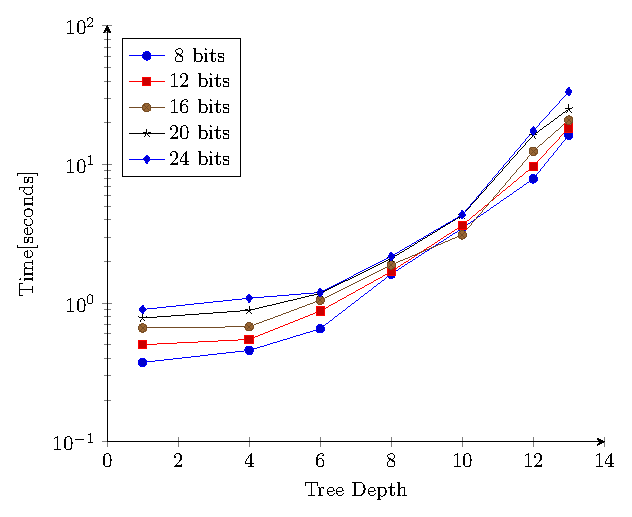
\includegraphics[height=6.1cm]{images/graphs/Pima_dt_gc.pdf}}%
\hspace{8pt}%
\subfigure[][]{%
\label{fig:dt-gc-BCWD}%
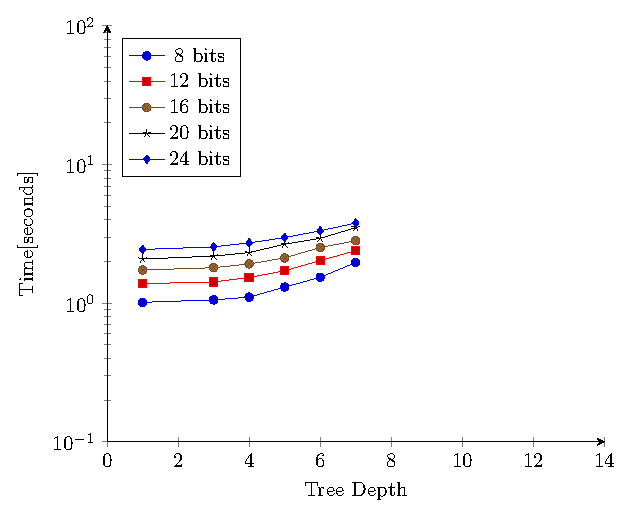
\includegraphics[height=6.1cm]{images/graphs/Breast_dt_gc.pdf}} \\
\subfigure[][]{%
\label{fig:dt-gc-CAD}%
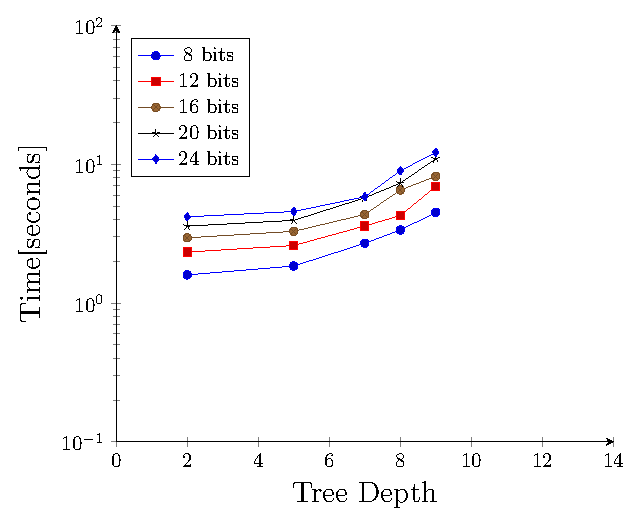
\includegraphics[height=6.1cm]{images/graphs/credit_dt_gc.pdf}}%
\hspace{8pt}%
\subfigure[][]{%
\label{fig:dt-gc-AID}%
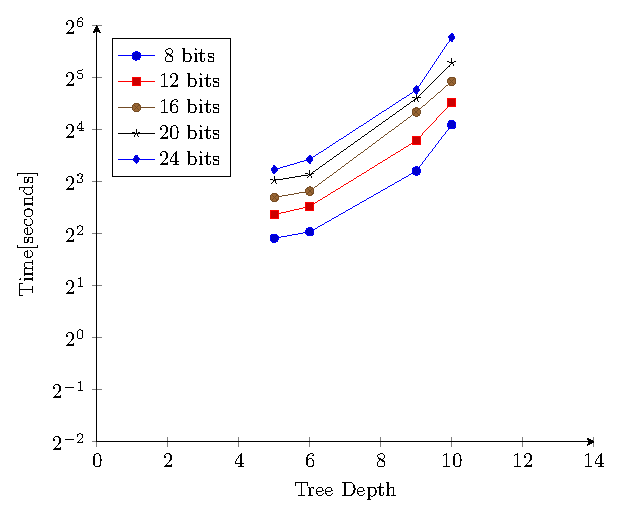
\includegraphics[height=6.1cm]{images/graphs/adult_dt_gc.pdf}}%
\caption[\acs{gc}+\acs{dt}. Runtime per data sample, in seconds. All datasets.]{\acs{gc}+\acs{dt}. Runtime per data sample, in seconds.
\subref{fig:dt-gc-pima} \emph{Pima Indians Diabetes} Dataset;
\subref{fig:dt-gc-BCWD} \emph{Breast Cancer Wisconsin Diagnostic} Dataset;
\subref{fig:dt-gc-CAD} \emph{Credit Approval} Dataset; and,
\subref{fig:dt-gc-AID} \emph{Adult Income} Dataset.}%
\label{fig:dt-gc}%
\end{figure}


Regarding the runtimes per data sample (Figure \ref{fig:dt-gc}), we can observe that the results obtained dominate over the pre-computation times. Although they scale slightly sub-linearly with the numeric precision and the number of features, they scale super-linearly with the number of nodes in the \ac{dt}. This can be a problem in terms of scalability since we are using fully expanded \ac{dt}, which means that increasing \ac{dt} depth leads to an exponential increase in the number of nodes. When comparing these results with those of the baseline, they are many orders of magnitude above, with the non-privacy-preserving approach in the order of milliseconds, and the privacy-preserving approach varying from seconds to hundreds of seconds. 
More detailed results are presented on Section \ref{app:gcdt_exec}.


\subsection{\acl{gc} and \acl{k-m}}
\label{ssec:gcandKM}


We present the execution times obtained by using the toolkit to build a \ac{gc} implementation of \ac{k-m} for all the datasets in the tables below. The results are presented in terms of average pre-computation times per data sample and runtimes per data sample. Table \ref{table:avgKMAllDatasets} presents the average pre-computation times for each data sample for all datasets. We can see that average pre-computation times are all very similar to one another despite the slight dependence on the \ac{gc} size, meaning that it does not impact the scalability of our solution.

\begin{table}[htp]
\centering
\caption{\acs{gc}+\acs{k-m}. Average pre-computation times per data sample, in seconds.}
\label{table:avgKMAllDatasets}
\vspace*{0.2cm}
\begin{tabular}{|l|r|r|r|r|r|}
\hline
\multirow{2}{*}{\textbf{Dataset}} & \multicolumn{5}{c|}{\textbf{Numeric Precision}}                                             \\ \cline{2-6} 
                                  & 8 bits & 12 bits & 16 bits & 20 bits & 24 bits \\ \hline
Pima                              & 0.260           & 0.283            & 0.307            & 0.331            & 0.339            \\ \hline
Breast                            & 0.225           & 0.251            & 0.274            & 0.289            & 0.301            \\ \hline
Credit                            & 0.226           & 0.249            & 0.253            & 0.265            & 0.272            \\ \hline
Adult                             & 0.214           & 0.214            & 0.232            & 0.266            & 0.262            \\ \hline
\end{tabular}
\end{table}

Regarding the runtimes per data sample (Figure \ref{fig:km-gc}), we observe again that the results are much larger that the pre-computation times. They scale linearly with the number of features and slightly super-linearly with the number of clusters, none of which compromises the scalability of our approach. However, runtimes scale quadratically with the numeric precision, which is caused by the multiplications required to compute the \ac{ed}. Although this causes scalability issues for large numeric precision, the results in Table \ref{table:avgErrorKM} show that the loss of accuracy is negligible even when only 12 bits are considered, allowing us to safely ignore this issue. The runtimes per data sample are also considerably large for the instances with a large number of clusters, but in our baseline system, we verified that the best results were always obtained when less than 10 clusters were considered. Even if this was not the case, we could sacrifice a small amount of accuracy by lowering the number of clusters considered in order to obtain much faster runtimes. When comparing these results with those of the baseline, they are many orders of magnitude above, with the non-privacy-preserving approach in the order of milliseconds, and the privacy-preserving approach varying from seconds to hundreds of seconds. Finally, it is important to mention that we did not compute all the entries in the tables above because the execution times for the larger datasets were becoming very long as the number of clusters and numeric precision grew and some examples were impossible to run due to insufficient RAM memory. More detailed results are presented on Section \ref{app:gckm_exec}.

\begin{figure}[t!]%
\centering
\subfigure[][]{%
\label{fig:km-gc-pima}%
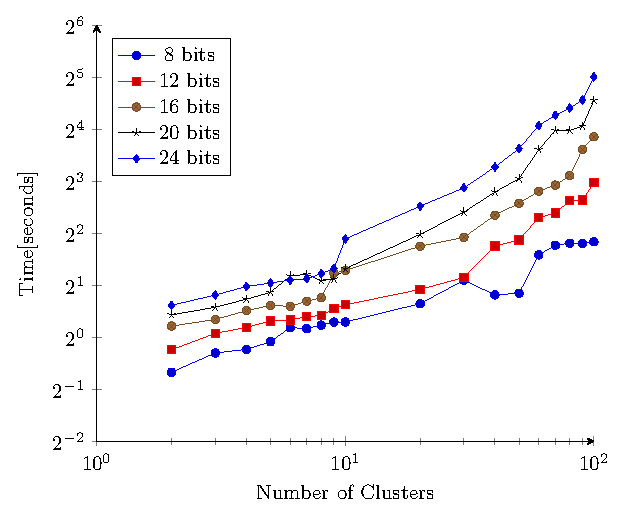
\includegraphics[height=6.1cm]{images/graphs/Pima_km_gc.pdf}}%
\hspace{8pt}%
\subfigure[][]{%
\label{fig:km-gc-BCWD}%
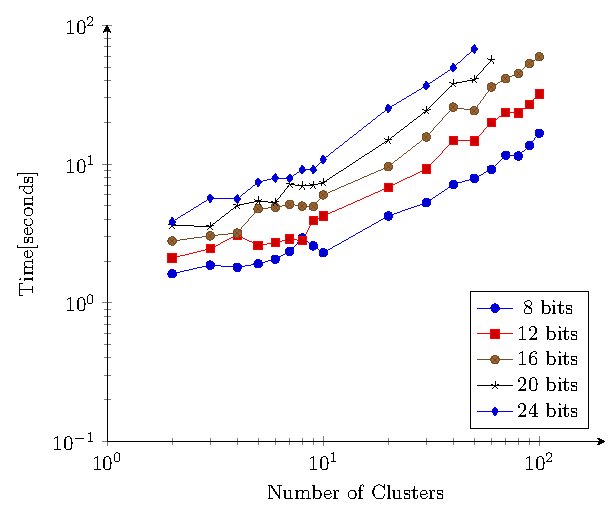
\includegraphics[height=6.1cm]{images/graphs/Breast_km_gc.pdf}} \\
\subfigure[][]{%
\label{fig:km-gc-CAD}%
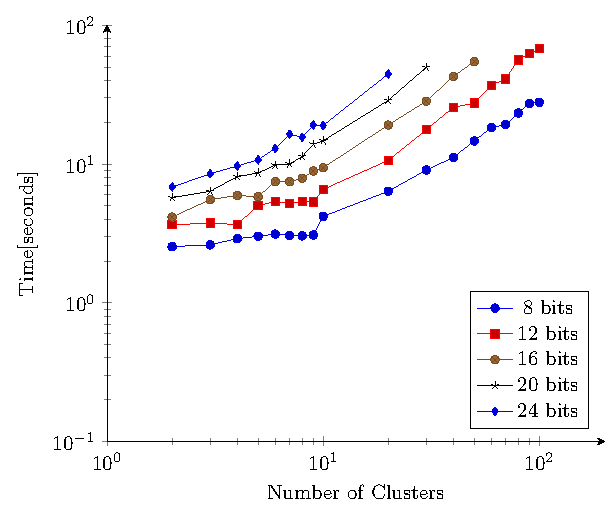
\includegraphics[height=6.1cm]{images/graphs/credit_km_gc.pdf}}%
\hspace{8pt}%
\subfigure[][]{%
\label{fig:km-gc-AID}%
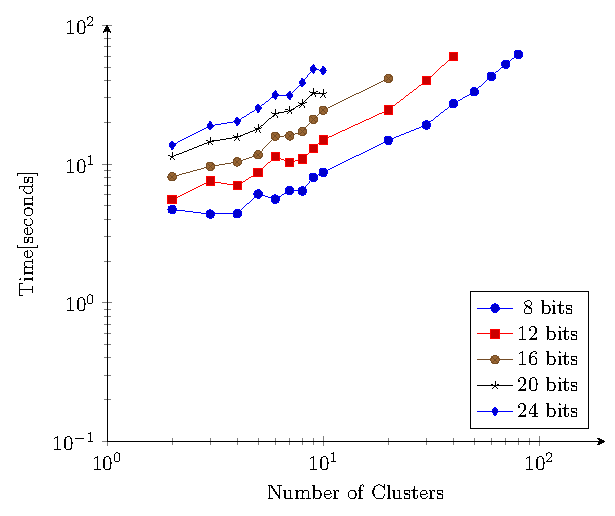
\includegraphics[height=6.1cm]{images/graphs/adult_km_gc.pdf}}%
\caption[\acs{gc}+\acs{k-m}. Runtime per data sample, in seconds. All datasets.]{\acs{gc}+\acs{k-m}. Runtime per data sample, in seconds.
\subref{fig:km-gc-pima} \emph{Pima Indians Diabetes} Dataset;
\subref{fig:km-gc-BCWD} \emph{Breast Cancer Wisconsin Diagnostic} Dataset;
\subref{fig:km-gc-CAD} \emph{Credit Approval} Dataset; and,
\subref{fig:km-gc-AID} \emph{Adult Income} Dataset.}%
\label{fig:km-gc}%
%\vspace*{-1.5cm}
\end{figure}


\subsection{\acl{he} and \acl{lr}}
\label{ssec:exec_he_lr}

%\vspace*{0.2cm}
As mentioned in Section \ref{sec:MyContributions}, the results presented in this section were developed by other team members in the \ac{bard} project at Altran, and are presented for completeness purposes.

\vspace*{0.4cm}
We present the execution times obtained by using the \ac{phe} and \ac{fhe} systems for all datasets in the tables below. For the \ac{fhe} system, we present the times for methods M1 and M2 in the same cell, for ease of comparison. The results are presented in terms of execution time per data sample. 

\begin{figure}[bh!]%
\vspace*{-0.2cm}
\centering
\subfigure[][]{%
\label{fig:lr-phe-pima}%
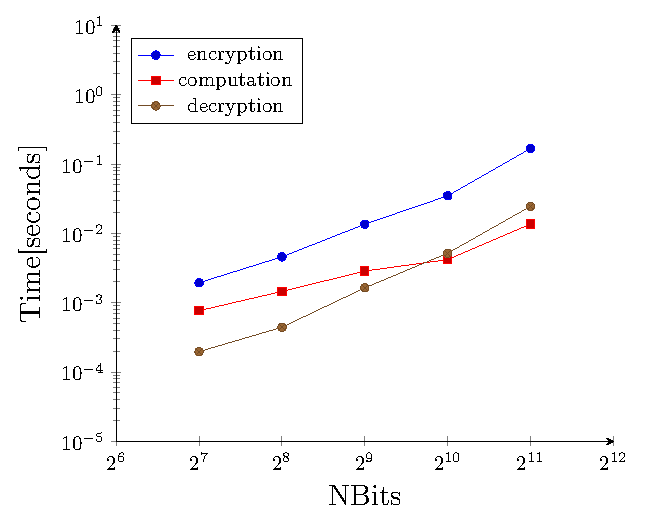
\includegraphics[height=6.1cm]{images/graphs/Pima_lr_phe.pdf}}%
\hspace{8pt}%
\subfigure[][]{%
\label{fig:lr-phe-BCWD}%
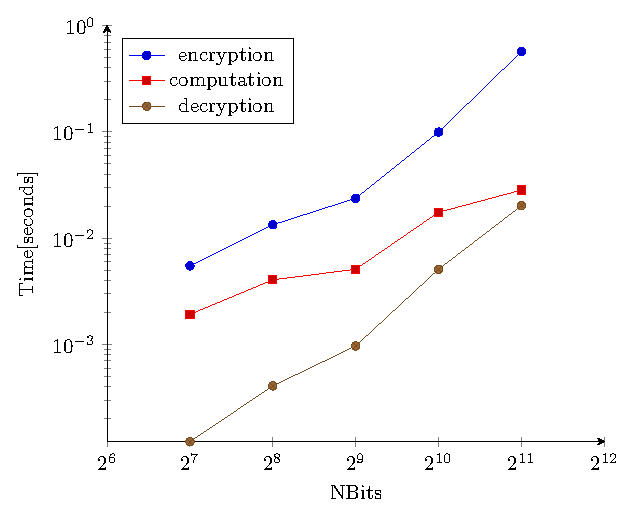
\includegraphics[height=6.1cm]{images/graphs/Breast_lr_phe.pdf}} \\
\subfigure[][]{%
\label{fig:lr-phe-CAD}%
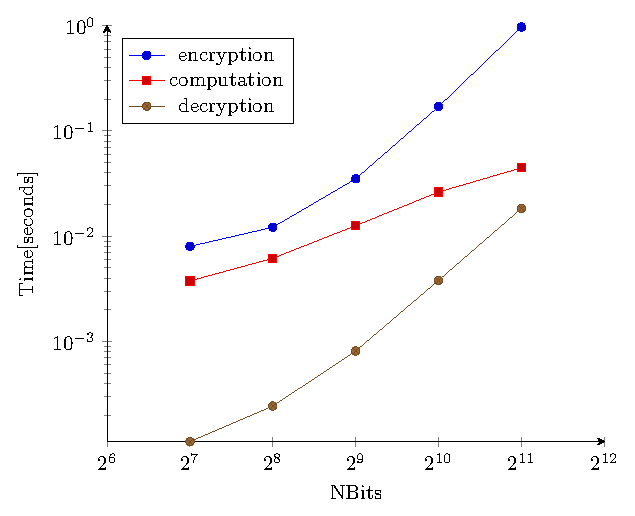
\includegraphics[height=6.1cm]{images/graphs/credit_lr_phe.pdf}}%
\hspace{8pt}%
\subfigure[][]{%
\label{fig:lr-phe-AID}%
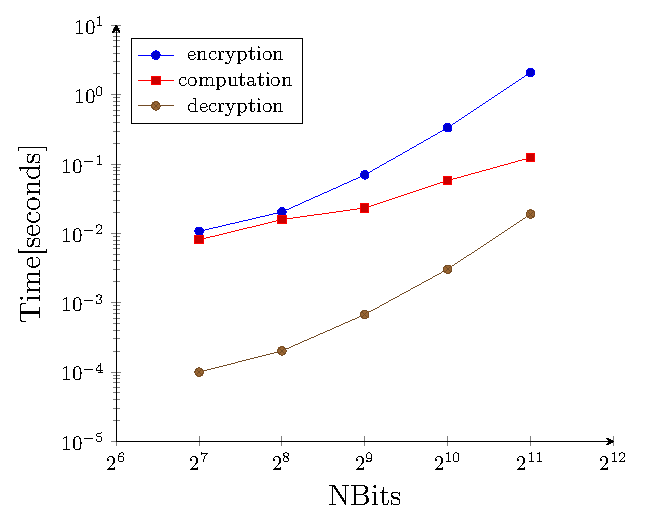
\includegraphics[height=6.1cm]{images/graphs/adult_lr_phe.pdf}}%
\caption[\acs{phe}+\acs{lr}. Execution time per data sample, in seconds. All datasets.]{\acs{phe}+\acs{lr}. Execution time per data sample, in seconds.
\subref{fig:lr-phe-pima} \emph{Pima Indians Diabetes} Dataset;
\subref{fig:lr-phe-BCWD} \emph{Breast Cancer Wisconsin Diagnostic} Dataset;
\subref{fig:lr-phe-CAD} \emph{Credit Approval} Dataset; and,
\subref{fig:lr-phe-AID} \emph{Adult Income} Dataset.}%
\label{fig:lr-phe}%
\end{figure}


When observing the execution times obtained using \ac{phe} (Figure \ref{fig:lr-phe}), we see that a linear increase in encryption and computation times when the number of features in the samples increases, but a constant decryption time, independent of the number of features.
We can also observe a linear increase in computation times, and a super-linear increase in encryption and decryption times, when the value of NBits increases. This can cause a problem of scalability, but it can be safely ignored since the execution times per sample are still very small.  When comparing these results with those of the baseline, the non-privacy-preserving results are in the order of milliseconds, and the privacy-preserving approach varies from deciseconds ($10^{-1}$s) to seconds. More detailed results are presented on Section \ref{app:phelr_exec}.

\begin{figure}[b!]
\centering
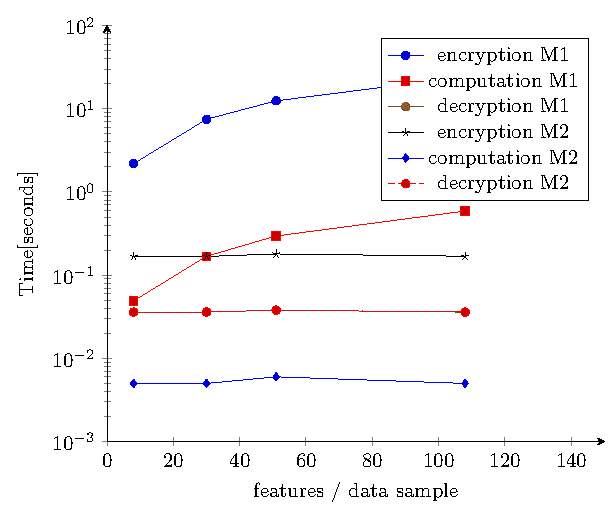
\includegraphics[width=0.65\textwidth]{images/graphs/lr_fhe.pdf}
\caption[\acs{fhe}+\acs{lr}. Execution time per data sample, in seconds. All datasets.]{\acs{fhe}+\acs{lr}. Execution time per data sample, in seconds. All Datasets.}
\label{fig:lr-fhe}
\end{figure}


When analyzing the results obtained using \ac{fhe} (Figure \ref{fig:lr-fhe}), we can observe that the packing used by method M2 greatly decreases the encryption and computation times, when compared to method M1. We also observe that method M2 makes the encryption and computation times independent from the number of features.
Overall, we see that method M2 is much more efficient that method M1, showing the obvious advantage of packing the features for each dataset in a single ciphertext before performing any computation. More detailed results are presented on Section \ref{app:fhelr_exec}.

When comparing \ac{phe} and \ac{fhe}, we observe that method M2 of \ac{fhe} has lower execution times than \ac{phe}, despite the complexity of the algorithm behind it. The only possible justification for this is the positive effect caused by feature packing, especially due to the gains in encryption time.




\subsection{\acl{he} and \acl{svm}}
\label{ssec:exec_he_svm}

\vspace*{-0.4cm}
Again, as mentioned in Section \ref{sec:MyContributions}, the results presented in this section were developed by other team members in the \ac{bard} project at Altran, and are presented for completeness purposes.

\vspace*{-0.2cm}
We present the execution times obtained by using the \ac{phe} and \ac{fhe} systems for all datasets in the tables below. Once again, for the \ac{fhe} system, we present the times for methods M1 and M2 in the same cell, for ease of comparison. The results are presented in terms of execution time per data sample for the \ac{phe} case, and execution time per sample and support vector for the \ac{fhe} case.

\begin{figure}[b!]%
\vspace*{-0.4cm}
\centering
\subfigure[][]{%
\label{fig:svm-phe-pima}%
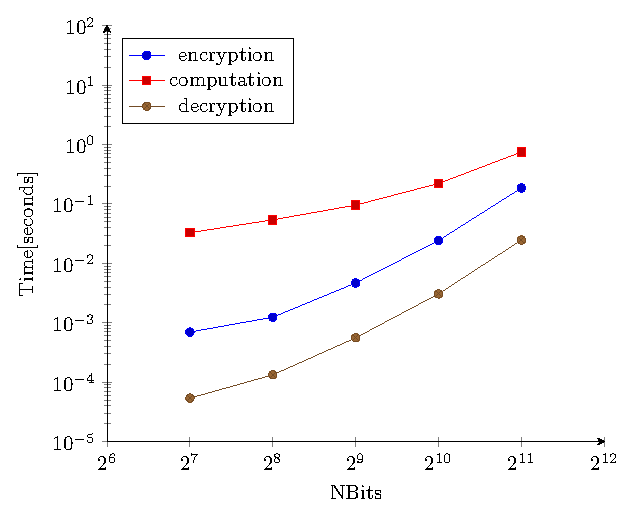
\includegraphics[height=6.1cm]{images/graphs/Pima_svm_phe.pdf}}%
\hspace{8pt}%
\subfigure[][]{%
\label{fig:svm-phe-BCWD}%
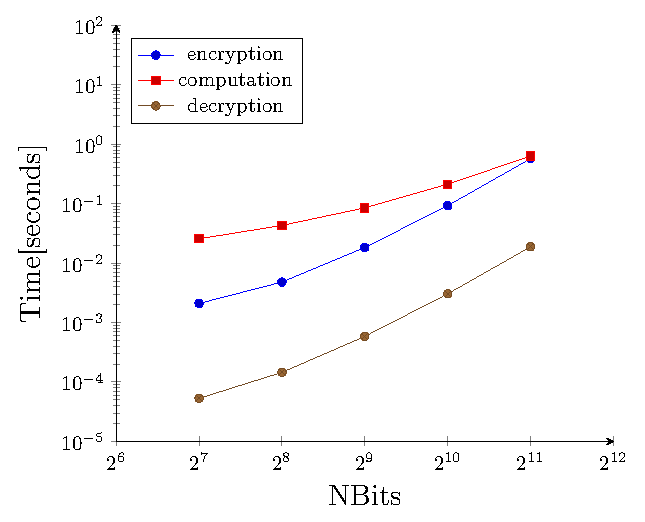
\includegraphics[height=6.1cm]{images/graphs/Breast_svm_phe.pdf}} \\
\vspace*{-0.2cm}
\subfigure[][]{%
\label{fig:svm-phe-CAD}%
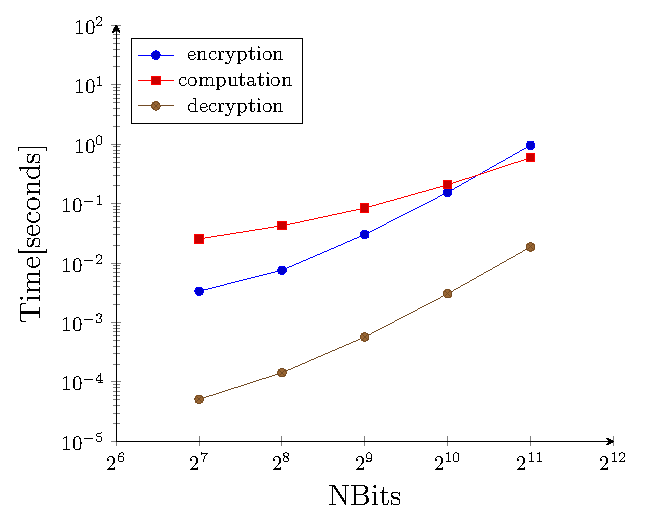
\includegraphics[height=6.1cm]{images/graphs/credit_svm_phe.pdf}}%
\hspace{8pt}%
\subfigure[][]{%
\label{fig:svm-phe-AID}%
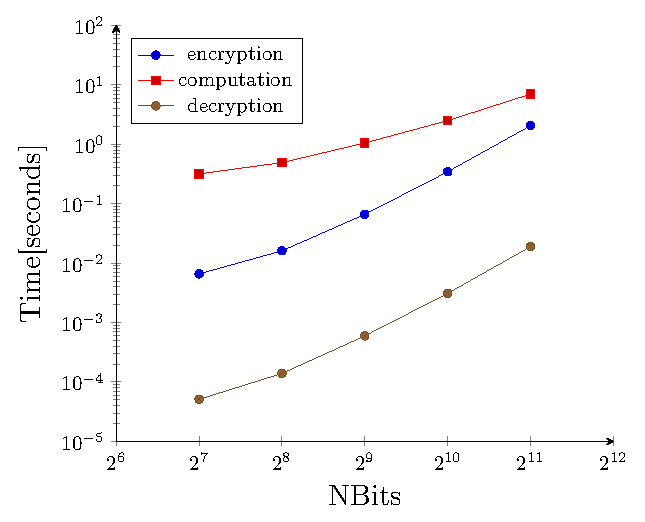
\includegraphics[height=6.1cm]{images/graphs/adult_svm_phe.pdf}}%
\vspace*{-0.2cm}
\caption[\acs{phe}+\acs{svm}. Execution time per data sample, in seconds. All datasets.]{\acs{phe}+\acs{svm}. Execution time per data sample, in seconds.
\subref{fig:svm-phe-pima} \emph{Pima Indians Diabetes} Dataset;
\subref{fig:svm-phe-BCWD} \emph{Breast Cancer Wisconsin Diagnostic} Dataset;
\subref{fig:svm-phe-CAD} \emph{Credit Approval} Dataset; and,
\subref{fig:svm-phe-AID} \emph{Adult Income} Dataset.}%
\label{fig:svm-phe}%
\vspace*{-0.3cm}
\end{figure}

When observing the execution times obtained using \ac{phe} (Figure \ref{fig:svm-phe}), we can see that computation times have a significant overhead for small amounts of number of features and number of Support Vectors, as they only affect the results in the \emph{Adult Income} Dataset, where they seem to have a linear dependency. 
We also observe a linear increase in encryption times with increasing the number of features and a linear increase in computation times with increasing NBits. When comparing these results with those of the baseline, the non-privacy-preserving results are in the order of milliseconds, and the privacy-preserving approach varies from deciseconds ($10^{-1}$s) to seconds.
Finally, we can see that decryption times are constant with increasing number of features and number of Support Vectors, but we verify that there is a slightly super-linear increase in encryption and decryption times with increasing NBits. This can cause a problem of scalability, but it can be safely ignored since the execution times per sample are still very small.
Additionally, for \ac{svm} we obtained similar encryption times to the ones obtained for \ac{lr}, which is not surprising since the encryption is only done on one side of the protocol (due to the way the Paillier cryptosystem works). Also, we can observe that decryption times are comparable in both cases, as decryption only occurs once, when all operations have been performed.
More detailed results are presented on Section \ref{app:phesvm_exec}.



\begin{figure}[b!]
\centering
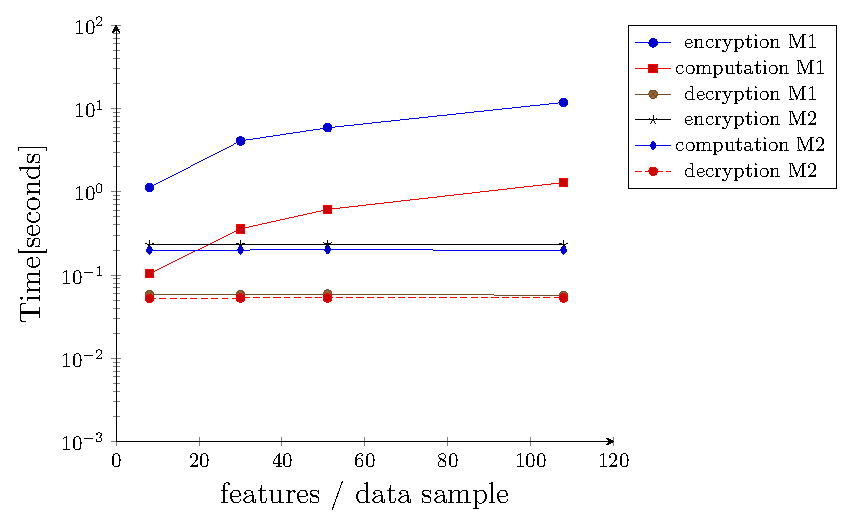
\includegraphics[width=0.60\textwidth]{images/graphs/svm_fhe.pdf}
\caption{\acs{fhe}+\acs{svm}. Execution time per data sample, in seconds. All datasets.}
\label{fig:svm-fhe}
\end{figure}

When observing the execution times obtained using \ac{fhe} (Figure \ref{fig:svm-fhe}), we can see similar results to those obtained for \ac{lr}. In particular, we see that the packing used by method M2 greatly decreases the encryption and computation times, when compared with method M1, as well as making the encryption and computation times independent from both the number of features and the number of Support Vectors. 
We can also observe that the decryption times are independent of the method used, the number of features and the number of Support Vectors. More detailed results are presented on Section \ref{app:fhesvm_exec}.

Once again, we can see that the method M2 is much more efficient than method M1, showing the obvious advantage of packing the features for each dataset in a single ciphertext before performing the computation. 

When comparing \ac{phe} and \ac{fhe}, unlike what was observed for \ac{lr}, here the former has lower execution times that the latter. Even considering the feature packing of method M2, the fact that many multiplications have to be made (one for each Support Vector) overwhelms \ac{fhe} when compared with \ac{phe} for evaluating an \ac{svm}.



%%%%%%%%%%%%%%%%%%%%%%%%%%%%%%%%%%%%%%%%%%%%%
\section{Communication Cost Results}
\label{sec:CommunicationCosts}
%%%%%%%%%%%%%%%%%%%%%%%%%%%%%%%%%%%%%%%%%%%%%%

As we will see in this Section, the communication cost is primarily defined by the cryptographic techniques considered and only secondarily by the \ac{ml} algorithms. We will focus on the former and address each of the specifics of the latter as needed. Given that cryptographic keys only need to be sent once and the ciphertext containing the desired result also only needs to be sent once, the bulk of the communication cost comes from the transmitting and receiving ciphertexts containing the actual data values. Since the amount of bytes sent by one of the parties is equal to the amount received by the other, and vice-versa, we will only present costs from one of the parties. We also do not present total communication costs for the whole datasets because communication costs per sample are independent of the dataset size, and communication costs per sample are the expected costs in a real-life scenario where a large computer cluster is available and data samples are supplied in a continuous fashion.


\subsection{\acl{gc} and \acl{dt}}

We present the communication costs obtained by using a \ac{gc} implementation of \ac{dt} for all datasets in the tables below. We present results in terms of average amount of bytes per data sample sent during pre-computation, received during pre-computation and sent during runtime, and the number of bytes per data sample received during runtime by the \ac{gc} evaluator.


\begin{table}[htp]
\centering
\caption{\acs{gc}+\acs{dt}. Average amount of bytes per data sample (in kB) sent during pre-computation (PC-S), received during pre-computation (PC-R) and sent during runtime (R-S) by the \ac{gc} evaluator. All datasets.}
\label{table:computationCostsDT}
\vspace*{0.2cm}
\begin{tabular}{|c|l|l|l|l|l|}
\hline
\multirow{2}{*}{\textbf{Dataset}} & \multicolumn{5}{c|}{\textbf{Numeric Precision}}  \\ \cline{2-6} 
 & \multicolumn{1}{c|}{8 bits}  & \multicolumn{1}{c|}{12 bits}   & \multicolumn{1}{c|}{16 bits}    & \multicolumn{1}{c|}{20 bits}  & \multicolumn{1}{c|}{24 bits} \\ \hline
Pima                     & \begin{tabular}[c]{@{}l@{}}PC-S: 1.055\\   PC-R: 2.342\\   R-S: 8.441\end{tabular}   & \begin{tabular}[c]{@{}l@{}}PC-S: 1.583\\   PC-R: 3.513\\   R-S: 12.662\end{tabular}  & \begin{tabular}[c]{@{}l@{}}PC-S: 2.110\\   PC-R: 4.685\\   R-S: 16.883\end{tabular}  & \begin{tabular}[c]{@{}l@{}}PC-S: 2.638\\   PC-R: 5.856\\   R-S: 21.104\end{tabular}  & \begin{tabular}[c]{@{}l@{}}PC-S: 3.166\\   PC-R: 7.027\\   R-S: 25.324\end{tabular}  \\ \hline
Breast                   & \begin{tabular}[c]{@{}l@{}}PC-S: 1.055\\   PC-R: 2.342\\   R-S: 31.656\end{tabular}  & \begin{tabular}[c]{@{}l@{}}PC-S: 1.583\\   PC-R: 3.514\\   R-S: 47.483\end{tabular}  & \begin{tabular}[c]{@{}l@{}}PC-S: 2.110\\   PC-R: 4.685\\   R-S: 63.311\end{tabular}  & \begin{tabular}[c]{@{}l@{}}PC-S: 2.638\\   PC-R: 5.856\\   R-S: 79.139\end{tabular}  & \begin{tabular}[c]{@{}l@{}}PC-S: 3.165\\   PC-R: 7.027\\   R-S: 94.967\end{tabular}  \\ \hline
Credit                   & \begin{tabular}[c]{@{}l@{}}PC-S: 1.055\\   PC-R: 2.342\\   R-S: 53.815\end{tabular}  & \begin{tabular}[c]{@{}l@{}}PC-S: 1.583\\   PC-R: 3.514\\   R-S: 80.722\end{tabular}  & \begin{tabular}[c]{@{}l@{}}PC-S: 2.110\\   PC-R: 4.685\\   R-S: 107.628\end{tabular} & \begin{tabular}[c]{@{}l@{}}PC-S: 2.638\\   PC-R: 5.812\\   R-S: 134.536\end{tabular} & \begin{tabular}[c]{@{}l@{}}PC-S: 3.166\\   PC-R: 7.027\\   R-S: 161.444\end{tabular} \\ \hline
Adult                    & \begin{tabular}[c]{@{}l@{}}PC-S: 1.055\\   PC-R: 2.342\\   R-S: 113.961\end{tabular} & \begin{tabular}[c]{@{}l@{}}PC-S: 1.583\\   PC-R: 3.514\\   R-S: 170.940\end{tabular} & \begin{tabular}[c]{@{}l@{}}PC-S: 2.110\\   PC-R: 4.685\\   R-S: 227.919\end{tabular} & \begin{tabular}[c]{@{}l@{}}PC-S: 2.638\\   PC-R: 5.855\\   R-S: 284.901\end{tabular} & \begin{tabular}[c]{@{}l@{}}PC-S: 3.166\\   PC-R: 7.027\\   R-S: 341.881\end{tabular} \\ \hline
\end{tabular}
\end{table}

\begin{figure}[!h]%
\centering
\subfigure[][]{%
\label{fig:dt-gc-comm-pima}%
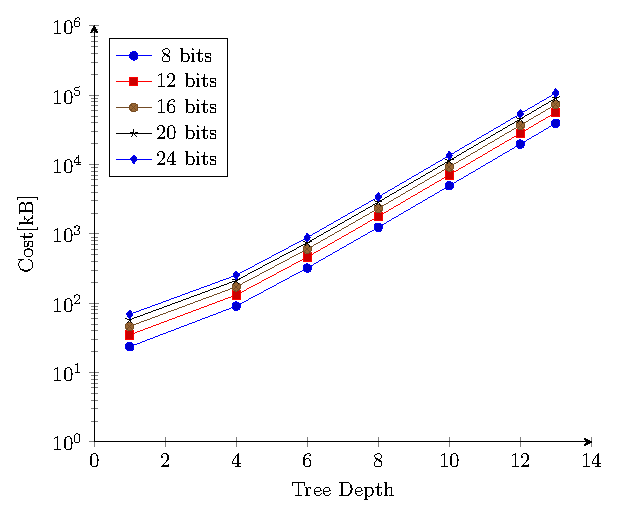
\includegraphics[height=6.1cm]{images/graphs/Pima_comm_dt_gc.pdf}}%
\hspace{8pt}%
\subfigure[][]{%
\label{fig:dt-gc-comm-BCWD}%
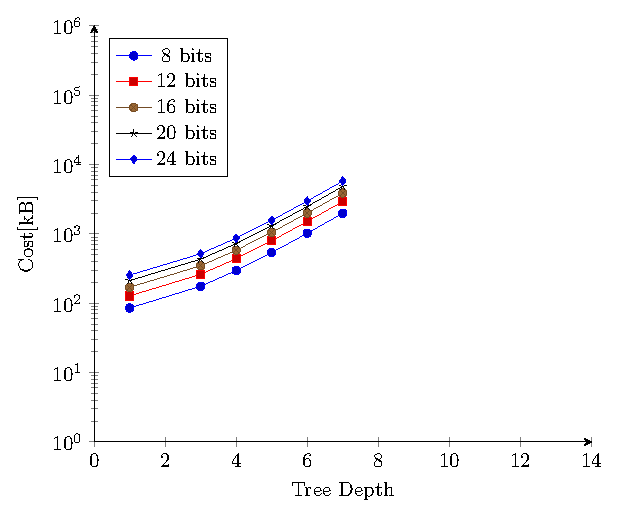
\includegraphics[height=6.1cm]{images/graphs/Breast_comm_dt_gc.pdf}} \\
\subfigure[][]{%
\label{fig:dt-gc-comm-CAD}%
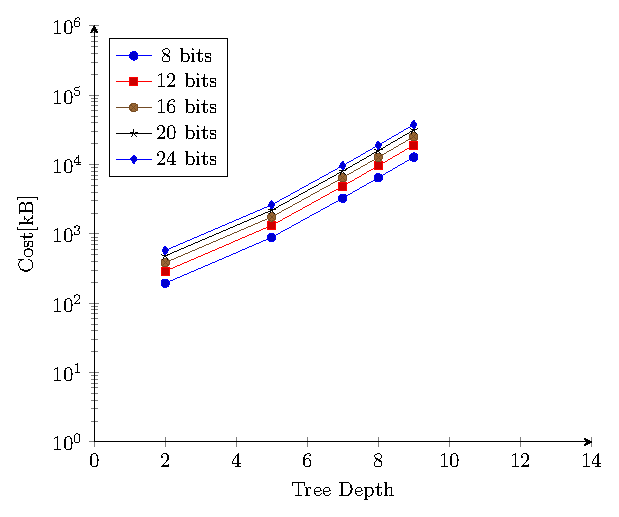
\includegraphics[height=6.1cm]{images/graphs/credit_comm_dt_gc.pdf}}%
\hspace{8pt}%
\subfigure[][]{%
\label{fig:dt-gc-comm-AID}%
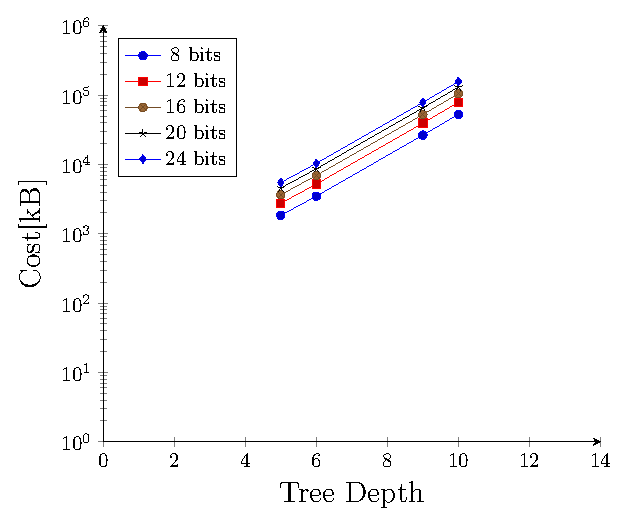
\includegraphics[height=6.1cm]{images/graphs/adult_comm_dt_gc.pdf}}%
\caption[\acs{gc}+\acs{dt}. Amount of bytes per data sample (in kB) received during runtime by the \ac{gc} evaluator. All datasets.]{\acs{gc}+\acs{dt}. Amount of bytes per data sample (in kB) received during runtime by the \ac{gc} evaluator.
\subref{fig:dt-gc-comm-pima} \emph{Pima Indians Diabetes} Dataset;
\subref{fig:dt-gc-comm-BCWD} \emph{Breast Cancer Wisconsin Diagnostic} Dataset;
\subref{fig:dt-gc-comm-CAD} \emph{Credit Approval} Dataset; and,
\subref{fig:dt-gc-comm-AID} \emph{Adult Income} Dataset.}%
\label{fig:dt-gc-comm}%
\end{figure}

In Table \ref{table:computationCostsDT}, we can see that all communication costs per data sample increase linearly with the variables of interest. Both the number of bytes sent and received by the \ac{gc} evaluator during pre-computation depend only on the numeric precision, and the amount of bytes sent during runtime depends only on the numeric precision and the number of features.

Regarding the amount of bytes per data sample received during runtime (Figure \ref{fig:dt-gc-comm}), they depend linearly on the numeric precision, on the number of features and on the number of \ac{dt} nodes, and therefore do not compromise the scalability of our approach. For larger \ac{dt}, the communication cost gets considerably large, but it can be easily minimized by using the original \ac{dt} instead of the fully expanded ones. More detailed results are presented on Section \ref{app:gcdt_comm}.




\subsection{\acl{gc} and \acl{k-m}}

We present the communication costs obtained by using a \ac{gc} implementation of \ac{k-m} for all datasets in the tables below. We present results in terms of the average number of bytes per data sample sent during pre-computation, received during pre-computation and sent during runtime, and the number of bytes per data sample received during runtime by the \ac{gc} evaluator. 


\begin{table}[htp]
\centering
\caption{\acs{gc}+\acs{k-m}. Average amount of bytes per data sample (in kB) sent during pre-computation (PC-S), received during pre-computation (PC-R) and sent during runtime (R-S) by the \ac{gc} evaluator. All datasets.}
\label{table:computationCostsKM}
\vspace*{0.2cm}
\begin{tabular}{|c|l|l|l|l|l|}
\hline
\multirow{2}{*}{\textbf{Dataset}} & \multicolumn{5}{c|}{\textbf{Numeric Precision}} \\ \cline{2-6} 
& \multicolumn{1}{c|}{8 bits}                                                 & \multicolumn{1}{c|}{12 bits}                                                & \multicolumn{1}{c|}{16 bits}                                                & \multicolumn{1}{c|}{20 bits}                                                & \multicolumn{1}{c|}{24 bits}                                                \\ \hline
Pima                     & \begin{tabular}[c]{@{}l@{}}PC-S: 1.055\\   PC-R: 2.342\\   R-S: 8.442\end{tabular}   & \begin{tabular}[c]{@{}l@{}}PC-S: 1.583\\   PC-R: 3.514\\   R-S: 12.662\end{tabular}  & \begin{tabular}[c]{@{}l@{}}PC-S: 2.110\\   PC-R: 4.685\\   R-S: 16.883\end{tabular}  & \begin{tabular}[c]{@{}l@{}}PC-S: 2.638\\   PC-R: 5.856\\   R-S: 21.104\end{tabular}  & \begin{tabular}[c]{@{}l@{}}PC-S: 3.166\\   PC-R: 7.027\\   R-S: 25.324\end{tabular}  \\ \hline
Breast                   & \begin{tabular}[c]{@{}l@{}}PC-S: 1.055\\   PC-R: 2.342\\   R-S: 31.656\end{tabular}  & \begin{tabular}[c]{@{}l@{}}PC-S: 1.583\\   PC-R: 3.514\\   R-S: 47.483\end{tabular}  & \begin{tabular}[c]{@{}l@{}}PC-S: 2.110\\   PC-R: 4.685\\   R-S: 63.311\end{tabular}  & \begin{tabular}[c]{@{}l@{}}PC-S: 2.638\\   PC-R: 5.856\\   R-S: 79.139\end{tabular}  & \begin{tabular}[c]{@{}l@{}}PC-S: 3.166\\   PC-R: 7.027\\   R-S: 94.967\end{tabular}  \\ \hline
Credit                   & \begin{tabular}[c]{@{}l@{}}PC-S: 1.055\\   PC-R: 2.342\\   R-S: 53.815\end{tabular}  & \begin{tabular}[c]{@{}l@{}}PC-S: 1.583\\   PC-R: 3.514\\   R-S: 80.722\end{tabular}  & \begin{tabular}[c]{@{}l@{}}PC-S: 2.110\\   PC-R: 4.685\\   R-S: 107.629\end{tabular} & \begin{tabular}[c]{@{}l@{}}PC-S: 2.638\\   PC-R: 5.856\\   R-S: 134.536\end{tabular} & \begin{tabular}[c]{@{}l@{}}PC-S: 3.166\\   PC-R: 7.027\\   R-S: 161.444\end{tabular} \\ \hline
Adult                    & \begin{tabular}[c]{@{}l@{}}PC-S: 1.055\\   PC-R: 2.342\\   R-S: 113.960\end{tabular} & \begin{tabular}[c]{@{}l@{}}PC-S: 1.583\\   PC-R: 3.514\\   R-S: 170.941\end{tabular} & \begin{tabular}[c]{@{}l@{}}PC-S: 2.110\\   PC-R: 4.685\\   R-S: 227.921\end{tabular} & \begin{tabular}[c]{@{}l@{}}PC-S: 2.638\\   PC-R: 5.856\\   R-S: 284.901\end{tabular} & \begin{tabular}[c]{@{}l@{}}PC-S: 3.166\\   PC-R: 7.027\\   R-S: 341.881\end{tabular} \\ \hline
\end{tabular}
\end{table}



\begin{figure}[!h]%
\centering
\subfigure[][]{%
\label{fig:km-gc-comm-pima}%
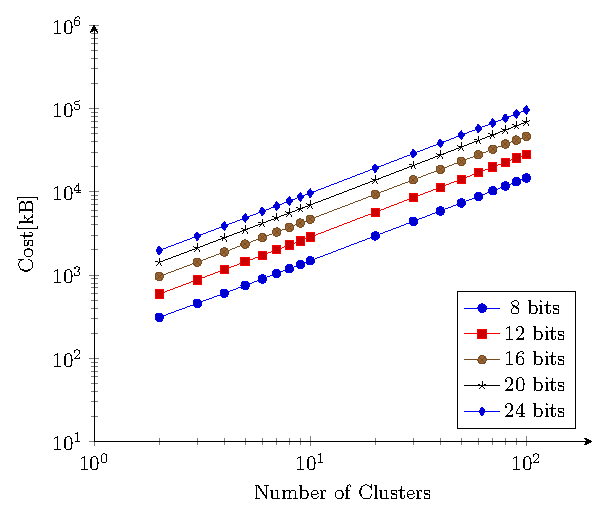
\includegraphics[height=6.1cm]{images/graphs/Pima_comm_km_gc.pdf}}%
\hspace{8pt}%
\subfigure[][]{%
\label{fig:km-gc-comm-BCWD}%
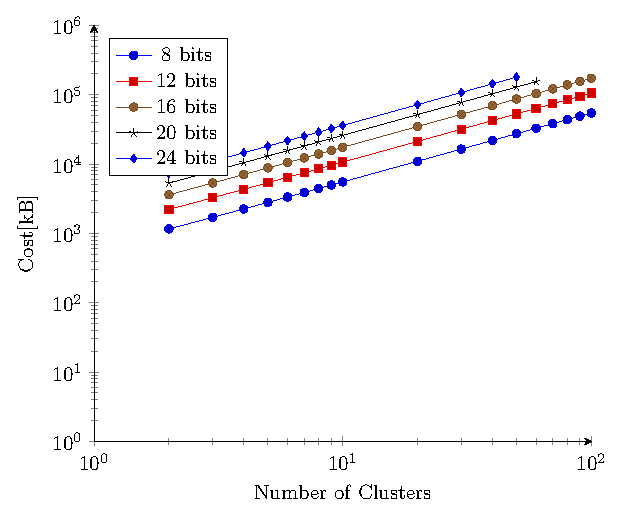
\includegraphics[height=6.1cm]{images/graphs/Breast_comm_km_gc.pdf}} \\
\vspace*{-0.2cm}
\subfigure[][]{%
\label{fig:km-gc-comm-CAD}%
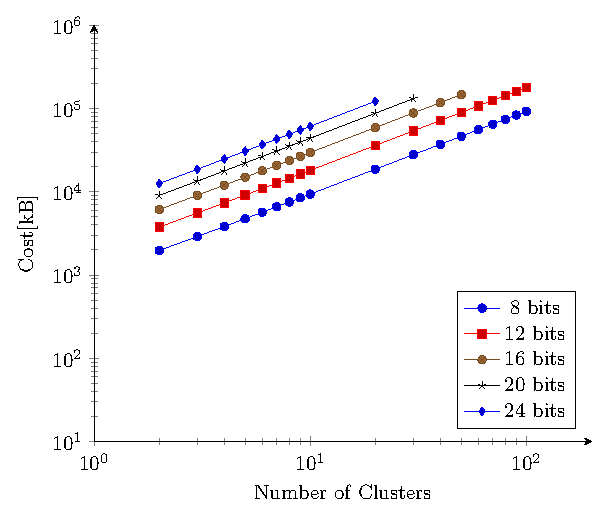
\includegraphics[height=6.1cm]{images/graphs/credit_comm_km_gc.pdf}}%
\hspace{8pt}%
\subfigure[][]{%
\label{fig:km-gc-comm-AID}%
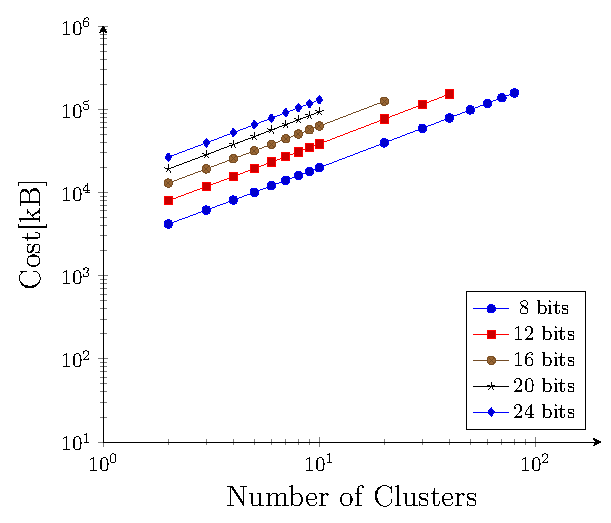
\includegraphics[height=6.1cm]{images/graphs/adult_comm_km_gc.pdf}}%
\vspace*{-0.2cm}
\caption[\acs{gc}+\acs{k-m}. Amount of bytes per data sample (in kB) received during runtime by the \ac{gc} evaluator. All datasets.]{\acs{gc}+\acs{k-m}. Amount of bytes per data sample (in kB) received during runtime by the \ac{gc} evaluator.
\subref{fig:km-gc-comm-pima} \emph{Pima Indians Diabetes} Dataset;
\subref{fig:km-gc-comm-BCWD} \emph{Breast Cancer Wisconsin Diagnostic} Dataset;
\subref{fig:km-gc-comm-CAD} \emph{Credit Approval} Dataset; and,
\subref{fig:km-gc-comm-AID} \emph{Adult Income} Dataset.}%
\label{fig:km-gc-comm}%
\vspace*{-0.2cm}
\end{figure}


In Table \ref{table:computationCostsKM}, we can see that all communication costs per data sample increase linearly with the variables of interest. Both the number of bytes sent and received by the \ac{gc} evaluator during pre-computation depend only on the numeric precision, and the amount of bytes sent during runtime depends only on the numeric precision and the number of features.

Regarding the amount of bytes per data sample received during runtime (Figure \ref{fig:km-gc-comm}), they depend linearly on the number of features and the number of clusters, and quadratically on the numeric precision. However, as we have seen before, the results on Table \ref{table:avgErrorKM} showed that the loss of accuracy is negligible even when only 12 bits are considered, meaning we can easily minimize its effects. Finally, it is important to mention that we did not compute all the entries in the tables above because the execution times for the larger datasets were becoming very long as the number of clusters and numeric precision grew and some examples were impossible to run due to insufficient RAM memory. More detailed results are presented on Section \ref{app:gckm_comm}.

%Tables \ref{table:computationCostsKM_PIMA}, \ref{table:computationCostsKM_BCWD}, \ref{table:computationCostsKM_CAD}, \ref{table:computationCostsKM_AID}, and 

\subsection{\acl{phe}}
\label{ssec:comm_phe}

As mentioned in Section \ref{sec:MyContributions}, the results presented in this section were developed in the \ac{bard} project at Altran, and are presented for completeness purposes.

For the \ac{phe} systems, both the key size and the ciphertexts size depend only on the number of bits chosen (NBits). For the Paillier cryptosystem in particular, both the public and private keys are composed of two $2*\text{NBits}$ numbers and any ciphertext is a $2*\text{NBits}$ number.

Under the assumption that one of the parties owns the data to be evaluated and the other owns the evaluation model and has the computational power to perform the evaluation, we only need to determine the communication cost of transmitting the data to be evaluated from one party to the other. This cost is independent of the \ac{ml} algorithm considered.

For each of the data samples, each individual feature value needs to be encrypted. The communication cost, in bits, is therefore given by:
\begin{equation}
\label{eq:PHE_commCost}
cost_{comm} = \underbrace{2(2\text{NBits})}_{\text{public key}} + \underbrace{Nn(2\text{NBits})}_{\text{ciphered data}} + \underbrace{2\text{NBits}}_{\text{ciphered result}} 
\end{equation}
where $N$ is the number of samples and $n$ is the number of features per sample.

As mentioned before, the ciphertexts containing the actual data overwhelm the other contributions. We present the communication costs for the datasets considered in Table \ref{table:PHECommCost}.

\begin{table}[htp]
\centering
\caption{\acs{phe}. Communication costs in kilobytes (kB). All datasets.}
\label{table:PHECommCost}
\vspace*{0.2cm}
\begin{tabular}{|c|r|r|r|r|}
\hline
\multirow{2}{*}{\textbf{NBits}} & \multicolumn{1}{c|}{\textbf{Pima}}          & \multicolumn{1}{c|}{\textbf{Breast Cancer}} & \multicolumn{1}{c|}{\textbf{Credit Approval}} & \multicolumn{1}{c|}{\textbf{Adult Income}}   \\ \cline{2-5}
                       & cost / sample & cost / sample & cost / sample   & cost / sample  \\ \hline
128       & 0.352        & 1.056          & 1.728          & 3.552         \\ \hline
256       & 0.704        & 2.112          & 3.456          & 7.104         \\ \hline
512       & 1.408        & 4.224          & 6.912          & 14.208        \\ \hline
1024      & 2.816        & 8.448          & 13.824         & 28.416        \\ \hline
2048      & 5.632        & 16.896         & 27.648         & 56.832        \\ \hline
\end{tabular}
\end{table}


As expected, the communication costs increase linearly with increasing NBits, the number of samples and the number of features. The communication costs for most datasets are considerably small, around a few megabytes. Even for the larger dataset, the \emph{Adult Income} Dataset, the larger costs are due only to the much higher number of samples considered; the cost per sample is still around a few kilobytes.



\subsection{\acl{fhe}}
\label{ssec:comm_fhe}

As mentioned in Section \ref{sec:MyContributions}, the results presented in this section were developed in the \ac{bard} project at Altran, and are presented for completeness purposes.

Considering the \ac{fhe} system used by the HElib toolkit, there was no easy way to precisely compute the total communication cost. The details of the cryptographic key generation process are not included in the toolkit documentation, and both the cryptographic keys and the ciphertexts are represented using their own structure. By printing several examples of cryptographic keys and ciphertexts, we estimated that each key is composed of approximately 400,000 64-bit values (total:$w_{key}\approx 3200\text{kB}=3.2\text{MB}$) and each ciphertext is composed of approximately 100,000 64-bit values (total:$w_{ciphertext}\approx 800\text{kB}=0.8\text{MB}$).

Under the assumption that one of the parties owns the data to be evaluated and the other owns the evaluation model and has the computational power to perform the evaluation, we only need to determine the communication cost of transmitting the data to be evaluated from one party to the other. This cost is independent of the \ac{ml} algorithm considered.

For each of the data samples, each individual feature value needs to be encrypted. The communication cost, in bits, is therefore given by:
\begin{equation}
\label{eq:FHE_commCost}
cost_{comm} = \underbrace{w_{key}}_{public key} + \underbrace{Nnw_{ciphertext}}_{ciphered data} + \underbrace{w_{ciphertext}}_{ciphered result}
\end{equation}
where $N$ is the number of samples and $n$ is the number of features per sample. As mentioned before, the ciphertexts containing the actual data overwhelm the other contributions. We present the communication costs for the datasets considered in Table \ref{table:FHECommCost}.


\begin{table}[htp]
\centering
\caption{\acs{fhe}. Communication costs in Megabytes (MB). All datasets.}
\label{table:FHECommCost}
\vspace*{0.2cm}
\begin{tabular}{|l|l|l|l|}
\hline
\textbf{Pima}          & \textbf{Breast Cancer} & \textbf{Credit Approval} & \textbf{Adult Income}   \\ \hline
cost / sample & cost / sample & cost / sample   & cost / sample  \\ \hline
10.4   & 28.0  & 44.8  & 90.4   \\ \hline
\end{tabular}
\end{table}

Once again, the communication costs increase linearly with increasing NBits, the number of samples and the number of features. However, we can observe the negative effect of the extremely long keys required by the \ac{fhe} system. The communication costs for all datasets are extremely high. Even if only a single data sample is considered, several megabytes are required for transmitting the corresponding ciphertext.



%%%%%%%%%%%%%%%%%%%%%%%%%%%%%%%%%%%%%%%%%%%%%
\section{Discussion}
\label{sec:ExperimentalResultsConclusion}
%%%%%%%%%%%%%%%%%%%%%%%%%%%%%%%%%%%%%%%%%%%%%%


We now make some final observations on the obtained results, analyzing the advantages and disadvantages of our \ac{gc} and \ac{he} approaches.

Although we did not compare the performance of \ac{gc} and \ac{he} directly, for instance by choosing a \ac{ml} algorithm and implementing it using both privacy-preserving techniques, it is clear that the \ac{he} approach is adequate for \ac{ml} algorithms that rely on arithmetic operations, and the \ac{gc} approach is adequate for \ac{ml} algorithms that rely on non-arithmetic operations. An example pointing in this direction is the quadratic increase in runtime verified in the \ac{gc}+\ac{k-m} experiments, due to the need to perform multiplications to compute the \ac{ed}.

An important remark on our experiments with \ac{gc} is related to our choice to only analyze fully expanded \ac{dt} instead of the original ones, in order to prevent any information leakage regarding the shape of the original tree. However, in most cases this causes an exponential growth of the number of nodes with increasing tree depths, leading to proportional increases in both the execution times and the communication costs.

We were also able to observe that the execution time increases by five orders of magnitude when comparing the baseline results with the privacy-preserving approach.

Another important conclusion with our experiments with \ac{he} is when each of the techniques should be used. We verified that \ac{phe} is, in fact, usable in practice but under some restrictions (e.g.: if there is no need for complex composition of operations and if data is separated between client and server), while \ac{fhe} is more flexible but still too computationally expensive. However, by using the coefficient packing in method M2, \ac{fhe} can be more efficient than \ac{phe} for evaluating some \ac{ml} algorithms (e.g.: \ac{lr}).



  %%%%%%%%%%%%%%%%%%%%%%%%%%%%%%%%%%%%%%%%%%%%%%%%%%%%%%%%%%%%%%%%%%%%%%%%%%%%%
  %
%%%%%                        LAST SECTION
 %%%
  %


%%%%%%%%%%%%%%%%%%%%%%%%%%%%%%%%%%%%%%%%%%%%%%
\section{Summary}
\label{sec:SummaryEvaluation}
%%%%%%%%%%%%%%%%%%%%%%%%%%%%%%%%%%%%%%%%%%%%%%


In this chapter, we detailed the experiments that were conducted in implementing our solution.
We presented the metrics used in evaluating the results obtained, as well as the setup and toolkits that were used to run the experiments.
The results we obtained using privacy-preserving algorithms, when compared with the ones obtained with the baseline, show that the loss of prediction performance is very small, as long as the numeric precision is 16 bits or more. 
We observed that \ac{ml} algorithms that rely on arithmetic operations have better performance with the \ac{he} approach. On the contrary, the \ac{gc} approach has better performance for \ac{ml} algorithms that rely on non-arithmetic operations.
We also observed the differences between \ac{phe} and \ac{fhe}, and were able to discern when each of the techniques should be used.





% In Section \ref{sec:EvaluationMetrics}, we presented the metric used in evaluating the results obtained.
% Section \ref{sec:ExperimentalSetup} detailed the setup that was used to run the experiments, as well as the toolkits used.
% In Section \ref{sec:ExperimentalResultsBaseline}, we presented the baseline results obtained for the datasets in question, and in Section \ref{sec:ExperimentalResultsComparisonBaseline} we compared those results with the ones obtained using the toolkits.
% In Section \ref{sec:ExperimentalResultsExecutionTime}, we presented the execution times for the implementation, and in Section \ref{sec:CommunicationCosts} we presented the communication costs for the implementation.
% Finally, in Section \ref{sec:ExperimentalResultsConclusion}, we made the final observations on the results obtained.


  %
 %%%
%%%%%                        THE END
  %
  %%%%%%%%%%%%%%%%%%%%%%%%%%%%%%%%%%%%%%%%%%%%%%%%%%%%%%%%%%%%%%%%%%%%%%%%%%%%%
